\documentclass{article}
\usepackage[margin=1.0in]{geometry}
\usepackage{titling}
\usepackage{graphicx}
\usepackage{float}
\usepackage[T1]{fontenc}

\begin{document}
	
	%%% title
	\setlength{\droptitle}{-5em}
	\title{3.7-8 Types of Triangles}
	\date{10-7-2020}
	\author{}
	\maketitle
	
	%%% first section
	\section{Angle Side Theorem}
	
\includegraphics[scale=0.8]{pics/T20.png}
	\newline \newline
	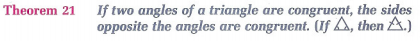
\includegraphics[scale=0.8]{pics/T21.png}
	\newline \newline
	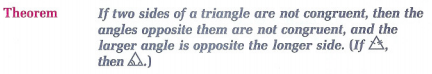
\includegraphics[scale=0.8]{pics/T21a.png}
	\newline \newline
	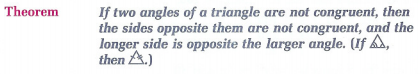
\includegraphics[scale=0.8]{pics/T21b.png}
	\newline \newline
	
	\section{Hypotenuse Leg (HL)}
	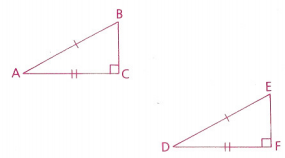
\includegraphics[scale=0.8]{pics/HL.png}
	\newline
	\textbf{POS: }If a correspondence exists between 2 $\triangle$s where the hyp $\cong$ and one leg of each is $\cong$ --> $\triangle \cong$
\end{document}